\documentclass[12pt,letterpaper]{article}
\usepackage{graphicx,textcomp}
\usepackage{natbib}
\usepackage{setspace}
\usepackage{fullpage}
\usepackage{color}
\usepackage[reqno]{amsmath}
\usepackage{amsthm}
\usepackage{fancyvrb}
\usepackage{amssymb,enumerate}
\usepackage[all]{xy}
\usepackage{endnotes}
\usepackage{lscape}
\newtheorem{com}{Comment}
\usepackage{float}
\usepackage{hyperref}
\newtheorem{lem} {Lemma}
\newtheorem{prop}{Proposition}
\newtheorem{thm}{Theorem}
\newtheorem{defn}{Definition}
\newtheorem{cor}{Corollary}
\newtheorem{obs}{Observation}
\usepackage[compact]{titlesec}
\usepackage{dcolumn}
\usepackage{tikz}
\usetikzlibrary{arrows}
\usepackage{multirow}
\usepackage{xcolor}
\usepackage{fancyvrb}
\newcolumntype{.}{D{.}{.}{-1}}
\newcolumntype{d}[1]{D{.}{.}{#1}}
\definecolor{light-gray}{gray}{0.65}
\usepackage{url}
\usepackage{listings}
\usepackage{color}
\usepackage{etoolbox}
\makeatletter
\preto{\@verbatim}{\topsep=0pt \partopsep=0pt }
\makeatother
\usepackage{placeins}



\definecolor{codegreen}{rgb}{0,0.6,0}
\definecolor{codegray}{rgb}{0.5,0.5,0.5}
\definecolor{codepurple}{rgb}{0.58,0,0.82}
\definecolor{backcolour}{rgb}{0.95,0.95,0.92}

\lstdefinestyle{mystyle}{
	backgroundcolor=\color{backcolour},   
	commentstyle=\color{codegreen},
	keywordstyle=\color{magenta},
	numberstyle=\tiny\color{codegray},
	stringstyle=\color{codepurple},
	basicstyle=\footnotesize,
	breakatwhitespace=false,         
	breaklines=true,                 
	captionpos=b,                    
	keepspaces=true,                 
	numbers=left,                    
	numbersep=5pt,                  
	showspaces=false,                
	showstringspaces=false,
	showtabs=false,                  
	tabsize=2
}
\lstset{style=mystyle}
\newcommand{\Sref}[1]{Section~\ref{#1}}
\newtheorem{hyp}{Hypothesis}


\title{Problem Set 3}
\date{Due: November 13, 2025}
\author{Ellen Beattie}


\begin{document}
	\maketitle
	\section*{Instructions}
	\begin{itemize}
		\item Please show your work! You may lose points by simply writing in the answer. If the problem requires you to execute commands in \texttt{R}, please include the code you used to get your answers. Please also include the \texttt{.R} file that contains your code. If you are not sure if work needs to be shown for a particular problem, please ask.
	\item Your homework should be submitted electronically on GitHub.
	\item This problem set is due before 23:59 on Thursday November 13, 2025. No late assignments will be accepted.

	\end{itemize}

		\vspace{.25cm}
	
\noindent In this problem set, you will run several regressions and create an add variable plot (see the lecture slides) in \texttt{R} using the \texttt{incumbents\_subset.csv} dataset. Include all of your code. \\

Loading in the dataset: 
\lstinputlisting[language=R, firstline=34, lastline=34]{EB_PS03.R}

	\vspace{.5cm}
\section*{Question 1}
\vspace{.25cm}
\noindent We are interested in knowing how the difference in campaign spending between incumbent and challenger affects the incumbent's vote share. 
		\begin{enumerate}
		\item Run a regression where the outcome variable is \texttt{voteshare} and the explanatory variable is \texttt{difflog}.	\vspace{1cm}
		
		Checking density plots, we do not see a significant skew in spread that may benefit from a transformation. 
		\lstinputlisting[language=R, firstline=38, lastline=40]{EB_PS03.R}
		
		The first model regresses voteshare on difflog (the difference in campaign spending between the incumbent and the challenger). 
		\lstinputlisting[language=R, firstline=43, lastline=50]{EB_PS03.R}
		% Table created by stargazer v.5.2.3 by Marek Hlavac, Social Policy Institute. E-mail: marek.hlavac at gmail.com
		% Date and time: Thu, Nov 13, 2025 - 09:08:16
		\begin{table}[!htbp] \centering 
			\caption{Incumbent/Challenger Difference in Campaign Spending
				on Incumbent's Voteshare} 
			\label{} 
			\begin{tabular}{@{\extracolsep{5pt}}lc} 
				\\[-1.8ex]\hline 
				\hline \\[-1.8ex] 
				& \multicolumn{1}{c}{\textit{Dependent variable:}} \\ 
				\cline{2-2} 
				\\[-1.8ex] & Voteshare \\ 
				\hline \\[-1.8ex] 
				Difference Log Spending & 0.042$^{***}$ \\ 
				& (0.001) \\ 
				& \\ 
				Constant & 0.579$^{***}$ \\ 
				& (0.002) \\ 
				& \\ 
				\hline \\[-1.8ex] 
				Observations & 3,193 \\ 
				R$^{2}$ & 0.367 \\ 
				Adjusted R$^{2}$ & 0.367 \\ 
				Residual Std. Error & 0.079 (df = 3191) \\ 
				F Statistic & 1,852.791$^{***}$ (df = 1; 3191) \\ 
				\hline 
				\hline \\[-1.8ex] 
				\textit{Note:}  & \multicolumn{1}{r}{$^{*}$p$<$0.1; $^{**}$p$<$0.05; $^{***}$p$<$0.01} \\ 
			\end{tabular} 
		\end{table} 
		\FloatBarrier
		
		\vspace{1cm}
		\item Make a scatterplot of the two variables and add the regression line.
		\lstinputlisting[language=R, firstline=53, lastline=60]{EB_PS03.R}
		\begin{figure}[!htbp]\centering
			\caption{\footnotesize Voteshare vs Difference Log}
			\label{fig:plot_4}
			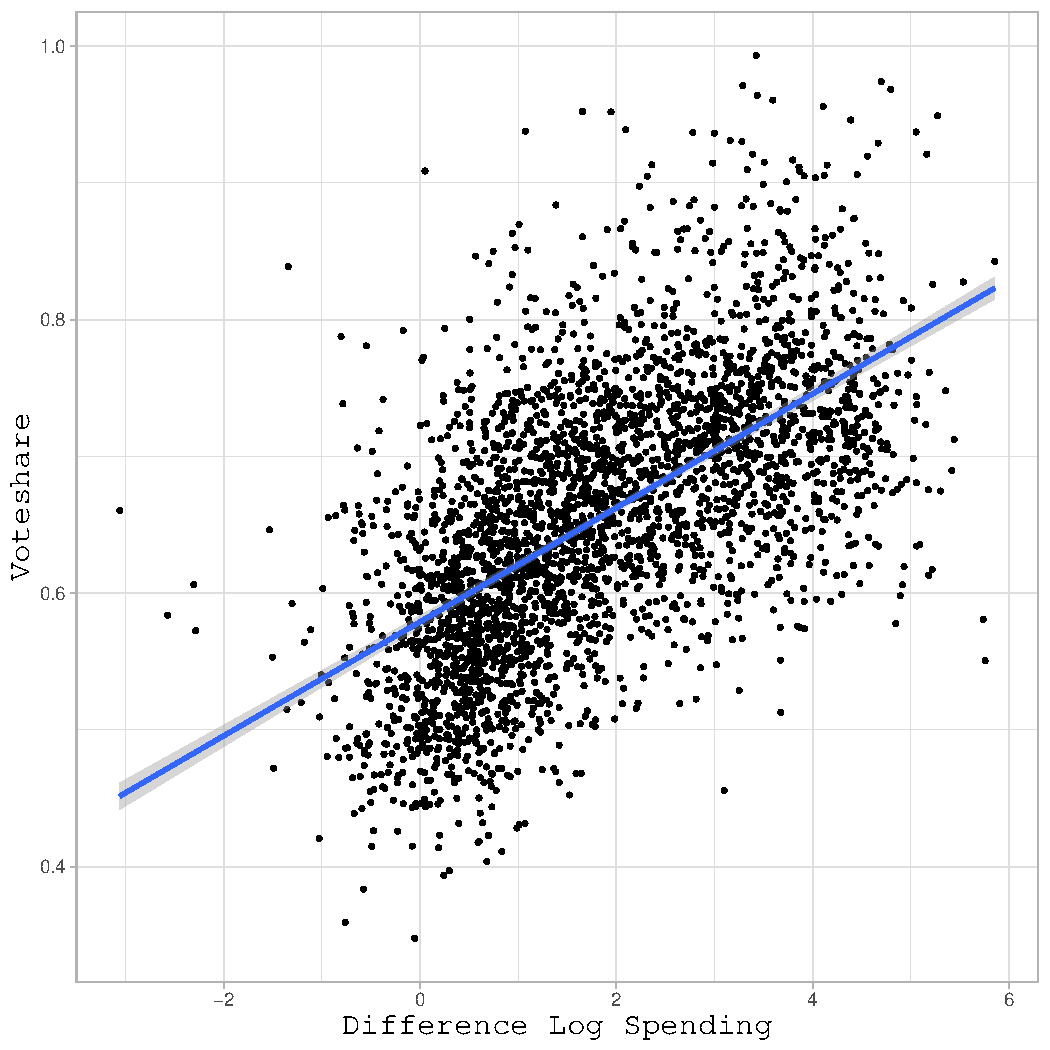
\includegraphics[width=.6\textwidth]{PS03_reg1plot.pdf}
		\end{figure}
		\FloatBarrier
		\item Save the residuals of the model in a separate object.	
		\lstinputlisting[language=R, firstline=63, lastline=63]{EB_PS03.R}
		\vspace{0.5cm}
		\item Write the prediction equation.
		\begin{equation}
			\widehat{\text{voteshare}} = 0.579+ 0.042\times\text{difflog}
		\end{equation}
		On average, a one unit increase in difflog is associated with a 0.042 increase in voteshare.
		\vspace{1cm}
		
	\end{enumerate}
	
\newpage

\section*{Question 2}
\noindent We are interested in knowing how the difference between incumbent and challenger's spending and the vote share of the presidential candidate of the incumbent's party are related.	\vspace{.25cm}
\begin{enumerate}
	\item Run a regression where the outcome variable is \texttt{presvote} and the explanatory variable is \texttt{difflog}.	
	\lstinputlisting[language=R, firstline=67, lastline=74]{EB_PS03.R}
	
	% Table created by stargazer v.5.2.3 by Marek Hlavac, Social Policy Institute. E-mail: marek.hlavac at gmail.com
	% Date and time: Thu, Nov 13, 2025 - 09:09:29
	\begin{table}[!htbp] \centering 
		\caption{Incumbent/Challenger Difference in Campaign Spending
			on the Presidential Candidate Voteshare of the Incumbent Party } 
		\label{} 
		\begin{tabular}{@{\extracolsep{5pt}}lc} 
			\\[-1.8ex]\hline 
			\hline \\[-1.8ex] 
			& \multicolumn{1}{c}{\textit{Dependent variable:}} \\ 
			\cline{2-2} 
			\\[-1.8ex] & Presidential Candidate Voteshare \\ 
			\hline \\[-1.8ex] 
			Difference Log & 0.024$^{***}$ \\ 
			& (0.001) \\ 
			& \\ 
			Constant & 0.508$^{***}$ \\ 
			& (0.003) \\ 
			& \\ 
			\hline \\[-1.8ex] 
			Observations & 3,193 \\ 
			R$^{2}$ & 0.088 \\ 
			Adjusted R$^{2}$ & 0.088 \\ 
			Residual Std. Error & 0.110 (df = 3191) \\ 
			F Statistic & 307.715$^{***}$ (df = 1; 3191) \\ 
			\hline 
			\hline \\[-1.8ex] 
			\textit{Note:}  & \multicolumn{1}{r}{$^{*}$p$<$0.1; $^{**}$p$<$0.05; $^{***}$p$<$0.01} \\ 
		\end{tabular} 
	\end{table} 
	\FloatBarrier
	\vspace{1cm}
	
	\item Make a scatterplot of the two variables and add the regression line. 
	\lstinputlisting[language=R, firstline=77, lastline=84]{EB_PS03.R}
	\begin{figure}[!htbp]\centering
		\caption{\footnotesize Presidential Voteshare vs Difflog}
		\label{fig:plot_2}
		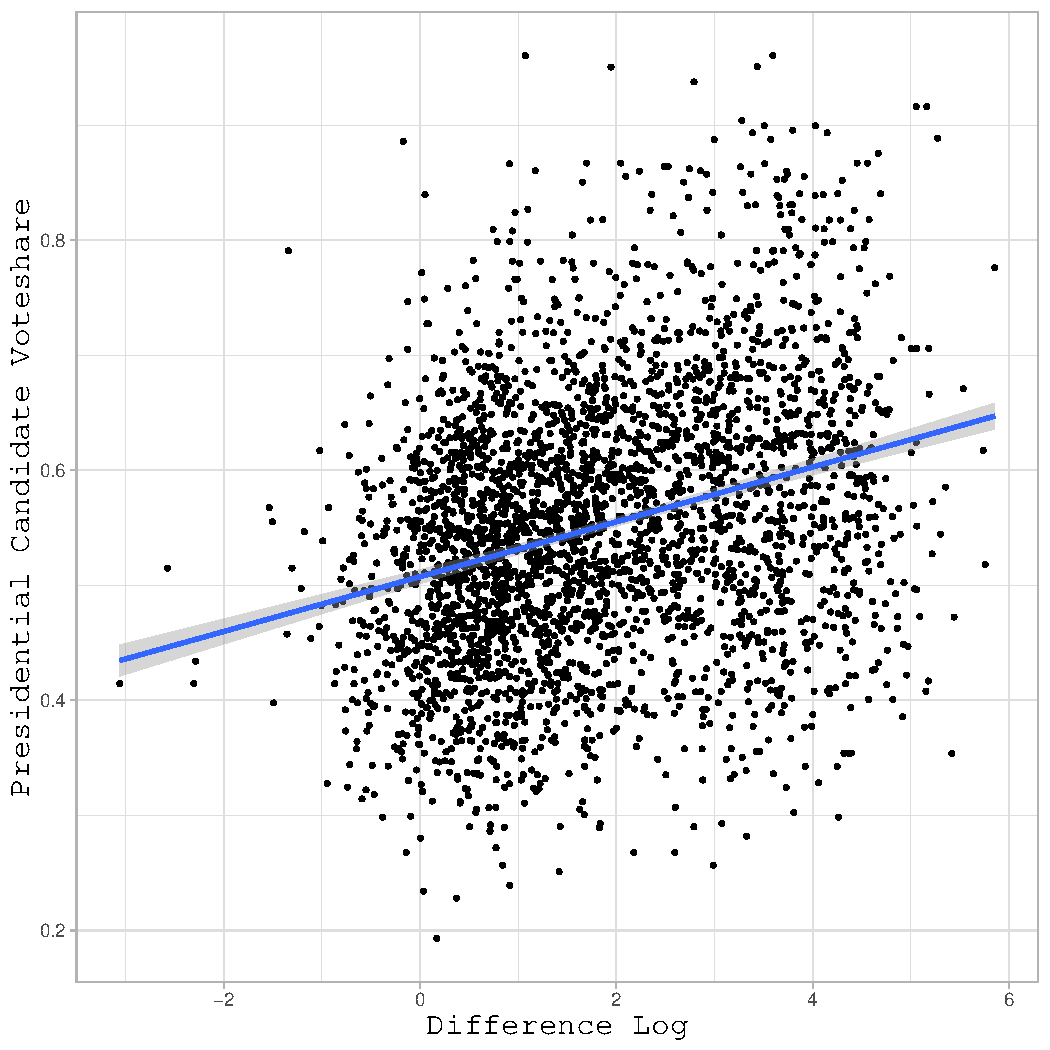
\includegraphics[width=.6\textwidth]{PS03_reg2plot.pdf}
	\end{figure}
	\FloatBarrier
	\vspace{1cm}
	\item Save the residuals of the model in a separate object.
	\lstinputlisting[language=R, firstline=87, lastline=87]{EB_PS03.R}
	\vspace{0.5cm}
	\item Write the prediction equation.
	\begin{equation}
		\widehat{\text{presvote}} = 0.508 + 0.024\times\text{difflog}
	\end{equation}
	On average, a one unit increase in difflog is associated with an 0.024 increase in presidential voteshare of incumbent's party.
	\vspace{1cm}
\end{enumerate}

\newpage	
\section*{Question 3}

\noindent We are interested in knowing how the vote share of the presidential candidate of the incumbent's party is associated with the incumbent's electoral success.
\vspace{.25cm}
\begin{enumerate}
	\item Run a regression where the outcome variable is \texttt{voteshare} and the explanatory variable is \texttt{presvote}.
	\lstinputlisting[language=R, firstline=91, lastline=98]{EB_PS03.R}
	
	% Table created by stargazer v.5.2.3 by Marek Hlavac, Social Policy Institute. E-mail: marek.hlavac at gmail.com
	% Date and time: Thu, Nov 13, 2025 - 09:11:19
	\begin{table}[!htbp] \centering 
		\caption{Presidential Candidate Voteshare of the Incumbent Party
			on the Incumbent's Voteshare} 
		\label{} 
		\begin{tabular}{@{\extracolsep{5pt}}lc} 
			\\[-1.8ex]\hline 
			\hline \\[-1.8ex] 
			& \multicolumn{1}{c}{\textit{Dependent variable:}} \\ 
			\cline{2-2} 
			\\[-1.8ex] & Voteshare \\ 
			\hline \\[-1.8ex] 
			Presidential Candidate Voteshare & 0.388$^{***}$ \\ 
			& (0.013) \\ 
			& \\ 
			Constant & 0.441$^{***}$ \\ 
			& (0.008) \\ 
			& \\ 
			\hline \\[-1.8ex] 
			Observations & 3,193 \\ 
			R$^{2}$ & 0.206 \\ 
			Adjusted R$^{2}$ & 0.206 \\ 
			Residual Std. Error & 0.088 (df = 3191) \\ 
			F Statistic & 826.950$^{***}$ (df = 1; 3191) \\ 
			\hline 
			\hline \\[-1.8ex] 
			\textit{Note:}  & \multicolumn{1}{r}{$^{*}$p$<$0.1; $^{**}$p$<$0.05; $^{***}$p$<$0.01} \\ 
		\end{tabular} 
	\end{table}
	\FloatBarrier
	\vspace{1cm}
	\item Make a scatterplot of the two variables and add the regression line. 
	\lstinputlisting[language=R, firstline=101, lastline=108]{EB_PS03.R}
	\begin{figure}[!htbp]\centering
		\caption{\footnotesize Voteshare vs Presidential Voteshare}
		\label{fig:plot_3}
		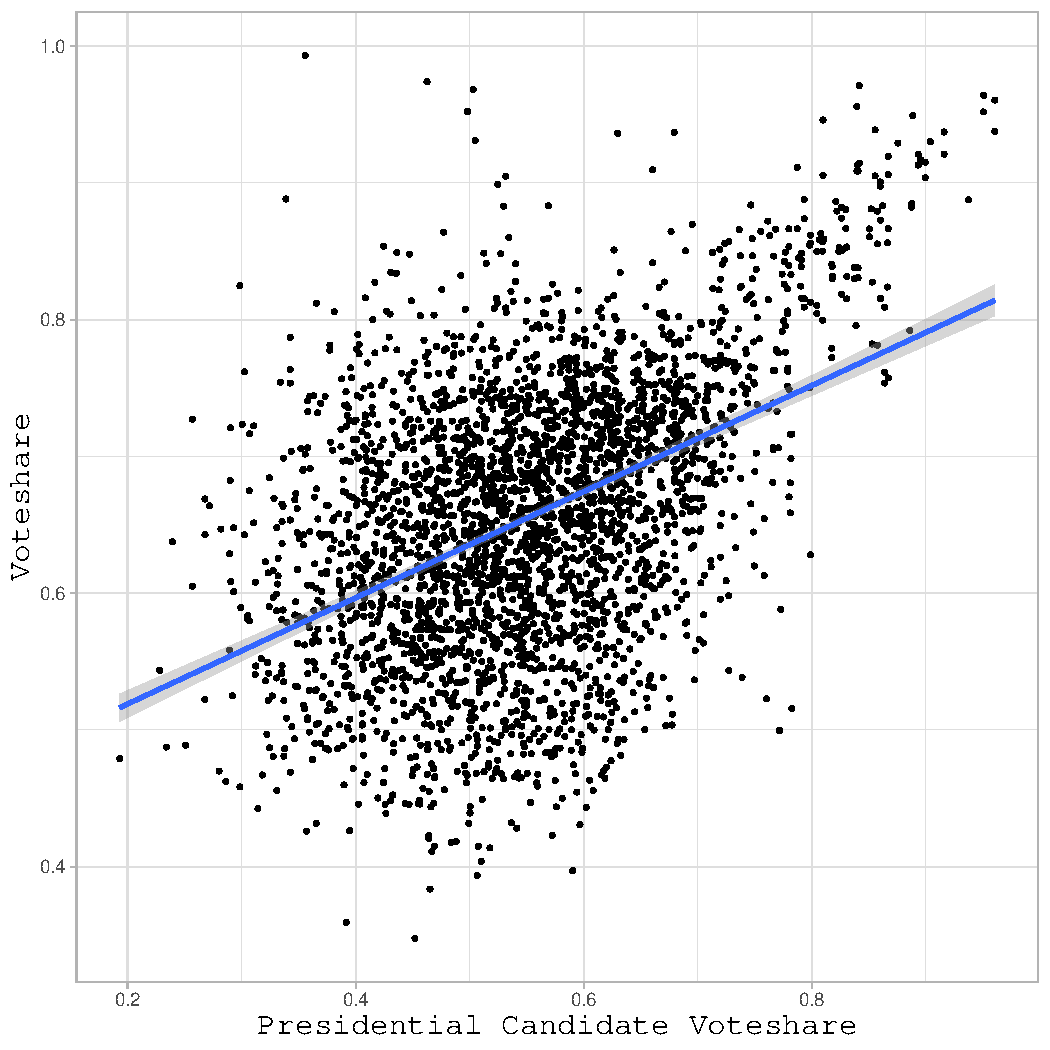
\includegraphics[width=.6\textwidth]{PS03_reg3plot.pdf}
	\end{figure}
	\FloatBarrier
	\vspace{1cm}
	\item Write the prediction equation.
	\begin{equation}
		\widehat{\text{voteshare}} = 0.441 + 0.388\times\text{presvote}
	\end{equation}
	On average, a one unit increase in presidential voteshare of incumbent's party is associated with an 0.388 increase in the incumbent's voteshare.
	\vspace{1cm}
\end{enumerate}


\newpage	
\section*{Question 4}
\noindent The residuals from part (a) tell us how much of the variation in \texttt{voteshare} is $not$ explained by the difference in spending between incumbent and challenger. The residuals in part (b) tell us how much of the variation in \texttt{presvote} is $not$ explained by the difference in spending between incumbent and challenger in the district.
\begin{enumerate}
	\item Run a regression where the outcome variable is the residuals from Question 1 and the explanatory variable is the residuals from Question 2.	
	\lstinputlisting[language=R, firstline=112, lastline=119]{EB_PS03.R}
	
	% Table created by stargazer v.5.2.3 by Marek Hlavac, Social Policy Institute. E-mail: marek.hlavac at gmail.com
	% Date and time: Thu, Nov 13, 2025 - 09:12:23
	\begin{table}[!htbp] \centering 
		\caption{Regression 1 Residuals on Regression 2 Residuals} 
		\label{} 
		\begin{tabular}{@{\extracolsep{5pt}}lc} 
			\\[-1.8ex]\hline 
			\hline \\[-1.8ex] 
			& \multicolumn{1}{c}{\textit{Dependent variable:}} \\ 
			\cline{2-2} 
			\\[-1.8ex] & Regression 1 Residuals \\ 
			\hline \\[-1.8ex] 
			Regression 2 Residuals & 0.257$^{***}$ \\ 
			& (0.012) \\ 
			& \\ 
			Constant & $-$0.000 \\ 
			& (0.001) \\ 
			& \\ 
			\hline \\[-1.8ex] 
			Observations & 3,193 \\ 
			R$^{2}$ & 0.130 \\ 
			Adjusted R$^{2}$ & 0.130 \\ 
			Residual Std. Error & 0.073 (df = 3191) \\ 
			F Statistic & 476.975$^{***}$ (df = 1; 3191) \\ 
			\hline 
			\hline \\[-1.8ex] 
			\textit{Note:}  & \multicolumn{1}{r}{$^{*}$p$<$0.1; $^{**}$p$<$0.05; $^{***}$p$<$0.01} \\ 
		\end{tabular} 
	\end{table}
	\FloatBarrier
	\vspace{1cm}
	\item Make a scatterplot of the two residuals and add the regression line. 
	\lstinputlisting[language=R, firstline=121, lastline=128]{EB_PS03.R}
	\begin{figure}[!htbp]\centering
		\caption{\footnotesize Regression 1 Residuals vs Regression 2 Residuals}
		\label{fig:plot_4}
		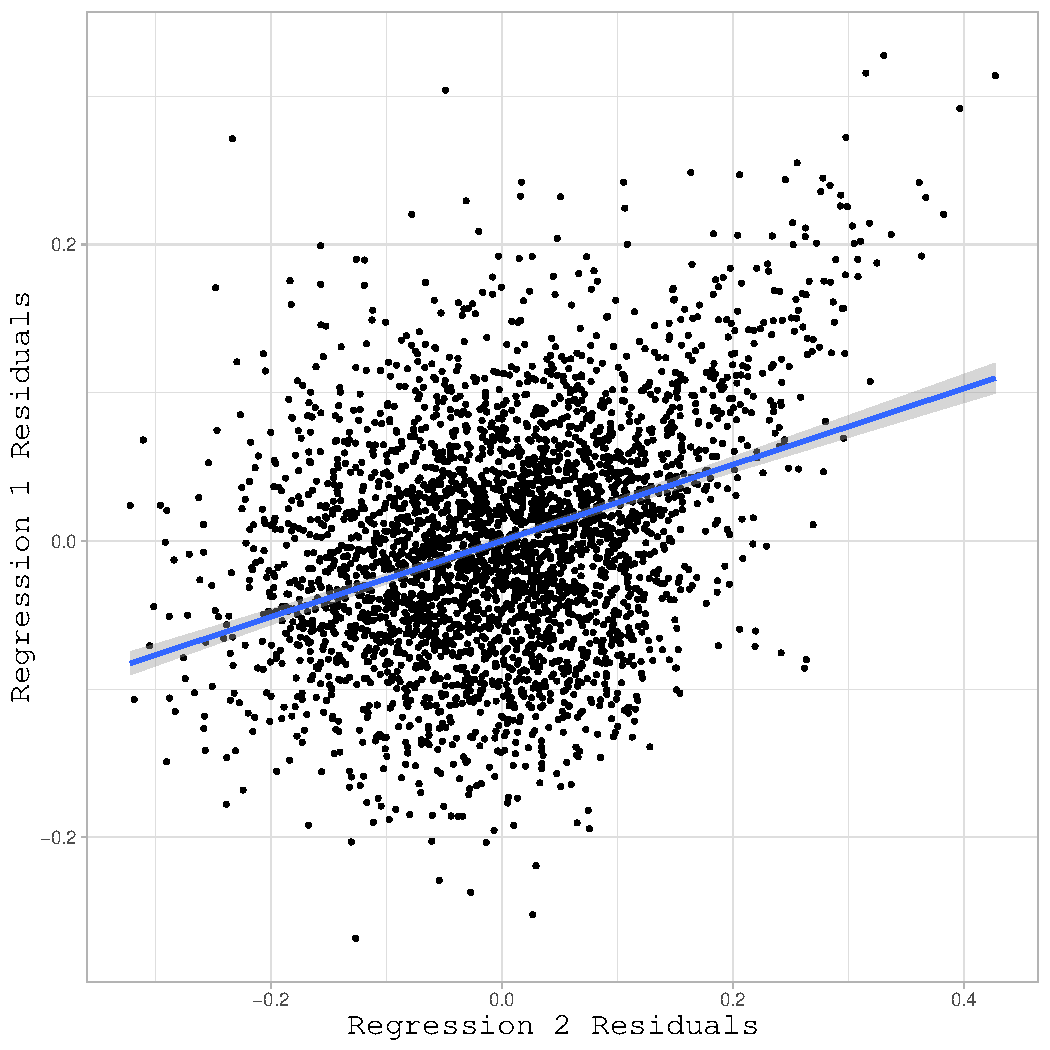
\includegraphics[width=.6\textwidth]{PS03_reg4plot.pdf}
	\end{figure}
	\FloatBarrier
	\vspace{1cm}
	\item Write the prediction equation.
	\begin{equation}
		\widehat{\text{reg1.residuals}} = -0.000 + 0.257\times\text{reg2.residuals}
	\end{equation}
	On average, a one unit increase in Regression 2 residuals is associated with an 0.257 increase in Regression 1 Residuals.\\
	That is, an increase in how much presvote variation is unexplained by difflog is associated with an 0.257 increase in how much voteshare variation is unexplained by difflog.
	
	\vspace{2cm}
\end{enumerate}


\section*{Question 5}
\noindent What if the incumbent's vote share is affected by both the president's popularity and the difference in spending between incumbent and challenger? 
\begin{enumerate}
	\item Run a regression where the outcome variable is the incumbent's \texttt{voteshare} and the explanatory variables are \texttt{difflog} and \texttt{presvote}.
	\lstinputlisting[language=R, firstline=132, lastline=140]{EB_PS03.R}
	
	% Table created by stargazer v.5.2.3 by Marek Hlavac, Social Policy Institute. E-mail: marek.hlavac at gmail.com
	% Date and time: Thu, Nov 13, 2025 - 09:13:00
	\begin{table}[!htbp] \centering 
		\caption{Incumbent/Challenger Difference in Campaign Spending and 
			the Presidential Candidate Voteshare of the Incumbent Party
			on the Incumbent's Voteshare} 
		\label{} 
		\begin{tabular}{@{\extracolsep{5pt}}lc} 
			\\[-1.8ex]\hline 
			\hline \\[-1.8ex] 
			& \multicolumn{1}{c}{\textit{Dependent variable:}} \\ 
			\cline{2-2} 
			\\[-1.8ex] & Voteshare \\ 
			\hline \\[-1.8ex] 
			Difference Log & 0.036$^{***}$ \\ 
			& (0.001) \\ 
			& \\ 
			Presidential Candidate Voteshare & 0.257$^{***}$ \\ 
			& (0.012) \\ 
			& \\ 
			Constant & 0.449$^{***}$ \\ 
			& (0.006) \\ 
			& \\ 
			\hline \\[-1.8ex] 
			Observations & 3,193 \\ 
			R$^{2}$ & 0.450 \\ 
			Adjusted R$^{2}$ & 0.449 \\ 
			Residual Std. Error & 0.073 (df = 3190) \\ 
			F Statistic & 1,302.947$^{***}$ (df = 2; 3190) \\ 
			\hline 
			\hline \\[-1.8ex] 
			\textit{Note:}  & \multicolumn{1}{r}{$^{*}$p$<$0.1; $^{**}$p$<$0.05; $^{***}$p$<$0.01} \\ 
		\end{tabular} 
	\end{table} 
	\FloatBarrier
	\vspace{1cm}
	\item Write the prediction equation.	
	\begin{equation}
		\widehat{\text{voteshare}} = 0.449+ 0.036\times\text{difflog} + 0.257\times\text{presvote}
	\end{equation}
	On average, a one unit increase in difflog is associated with a 0.036 increase in voteshare, holding all else constant. A one unit increase in presvote is, on average, associated with a 0.257 increase in voteshare, holding all else constant. 
	\vspace{1cm}
	\item What is it in this output that is identical to the output in Question 4? Why do you think this is the case? \\
	\begin{itemize}
		\item The regression coefficient of Presidential Vote share (0.257) in model 5 is the same as the regression coefficient of Regression 2 residuals in model 4.
		\item Model 4 regresses the reg1residuals (i.e. the part of voteshare unexplained by difflog) on reg2residuals (i.e. the part of Presidential voteshare unexplained by difflog).  
		\item Using the residuals that remove the effect of difflog on voteshare and on presvote, model 4 eliminates the confounding effect of difflog on both and computes the independent effect of presidential voteshare on voteshare.  
		\item This is ultimately the same process that occurs when running a multivariate regression, which statistically controls for the effect of other variables in the model. 
		\item In the multivariate model 5 the coefficient of presvote (0.257) is determined independent of the effect of the other explanatory variable difflog, and is therefore identical to that in model 4.
	\end{itemize}
	
	\vspace{1cm}
\end{enumerate}


\end{document}
